\chapter{Time-dependent Edge Cost Estimation}
Chapter~\ref{Ch:ldmk_graph} describes the general procedures for constructing a landmark graph. To find a time-dependent shortest route on a landmark graph, the time-dependent edge cost must be calculated. In this project, the time-dependent edge cost specifically refers to travel time, but in theory, it can refer to any quantity that can be described as a time-dependent edge cost function of the form $w : E,t \rightarrow \mathbb{R}$. In practice, it sometimes also refers to fuel consumptions or taxi fares. This chapter introduces a machine learning-based approach to estimate the travel time of each \emph{significant edge} in a landmark graph at a particular moment in time. 

\begin{defn}[\emph{Support}]
A support for an edge $e$ in a landmark graph $G=(V,E)$ is the number of times that $e$ appears. 
\end{defn}

\begin{defn}[\emph{Significant Edge}]
A significant edge in a landmark graph $G=(V,E)$ is an edge $e \in E$ that has a support at least $m$, where $m$ is a parameter specified in advance.
\end{defn}

The purpose of defining significant edges is to eliminate those edges that are seldom traversed by taxi drivers, as estimating the travel time of those edges will not be very accurate. The parameter $m$ also represents a level of \emph{confidence}, that is, to what extent it is true that this edge \emph{really} exists in the real world. 

Everyday experiences show that the travel time of a particular road usually has different time-varying patterns in weekdays as compared to that in weekends or public holidays. For instance, it is likely that, on weekdays, the travel time of a particular road has one \emph{peak} at 8 a.m. when people travel to work and the other peak at 6 p.m. when people return home after work. But when it is weekends or public holidays, the travel time of that road may have a peak at 10 a.m. when people go for holiday activities with families and the other peak at only about 8 p.m. when the whole day's celebrations are over. 

Based on this intuition, two separate landmark graphs were built in this project, with one for weekdays and the other for weekends or public holidays. Moreover, as mentioned in Section~\ref{Subsec:outlier_removal}, 
two data sets, bjtaxigps\_30m and bjtaxigps\_50m, remained after outlier removal based on different thresholds set for removing outliers. Therefore, in total, \emph{four} landmark graphs were built in this project and they are summarised in Table~\ref{Ta:ldmkgraphs}, although their names are self-explanatory. 

\begin{table}[h!]
\centering
\resizebox{\columnwidth}{!}{
\begin{tabular}{ | c | c | }
\hline
\textbf{Landmark Graph} & \textbf{Data Source} \\ \hline
wrkd\_ldmkgraph\_30m & weekday trajectories in bjtaxigps\_30m\\\hline
holi\_ldmkgraph\_30m & holiday trajectories in bjtaxigps\_30m \\\hline
wrkd\_ldmkgraph\_50m & weekday trajectories in bjtaxigps\_50m\\\hline
holi\_ldmkgraph\_50m  & holiday trajectories in bjtaxigps\_50m\\ \hline
\end{tabular}}
\caption{An summary of landmark graphs}\label{Ta:ldmkgraphs}
\end{table}

\section{Travel Time Distribution}
\begin{figure}[h!]
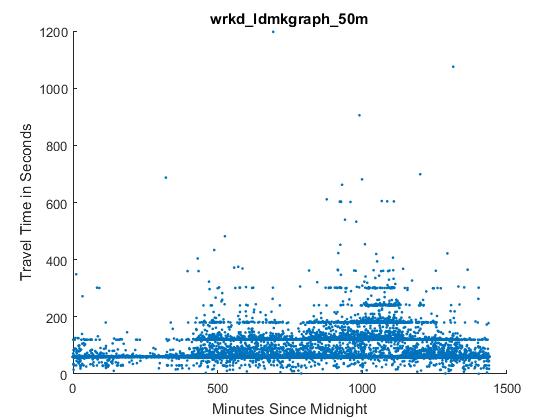
\includegraphics[scale=0.85]{trvltime_scatter}
\centering
\caption{An example of travel time patterns}\label{Fig:wrkd_50m_trvltime}
\end{figure}

Figure~\ref{Fig:wrkd_50m_trvltime} illustrates a scatter plot of the travel time of a particular landmark graph edge during the course of a weekday. It can be observed that the travel time does not seem to be a single-valued function with respect to time of the day, as one may expect; rather, the scatter points tend to gather around some values and form some \emph{clusters}. For instance, when it is 500 minutes since midnight, namely 8:20~a.m., the travel time seems to have three main clusters which are represented by three horizontal lines formed by the scatter points. When it is 1,000 minutes since midnight, namely 4:40~p.m., there are about five such lines. This pattern is attributable to three possible reasons:
\begin{enumerate}
\item Drivers may actually choose different routes to travel between the two landmarks, which cannot be captured by the landmark graph since it only knows a driver has traversed between the two landmarks but not the exact route. Different routes have different traffic conditions and speed limitations, therefore the travel time varies;
\item Drivers have different driving skills, preferences and behaviours. Some drivers just drive faster than others, even if the road conditions are similar and;
\item The GPS devices on taxis reported locations \emph{periodically}, therefore, durations like 60 seconds or 120 seconds are very commonly seen in the landmark graphs. Even if the \emph{actual} travel time is 53 seconds, it is still recorded as 60 seconds. This corresponds to the low-sampling-rate problem mentioned in Section~\ref{Sec:limitation}. 
\end{enumerate}

\begin{figure}[h!]
\centering
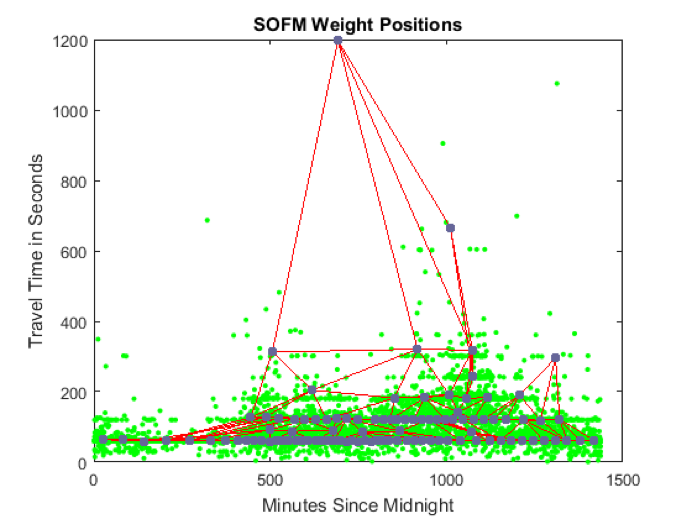
\includegraphics[scale=0.85]{trvltime_clus} 
\caption{Final positions of the neurons}\label{Fig:trvltime_clus}
\end{figure}

Therefore, it is not possible to fit the scatter points with a single-valued function. Rather, the clustering technique should first be employed to identify the travel time clusters. Like in Section~\ref{SubSec:outlier_identify}, a \textbf{self-organising feature map} is used to cluster the scatter points. Figure~\ref{Fig:trvltime_clus} shows the final positions of the neurons at the end of the training.

\begin{figure}[h!]
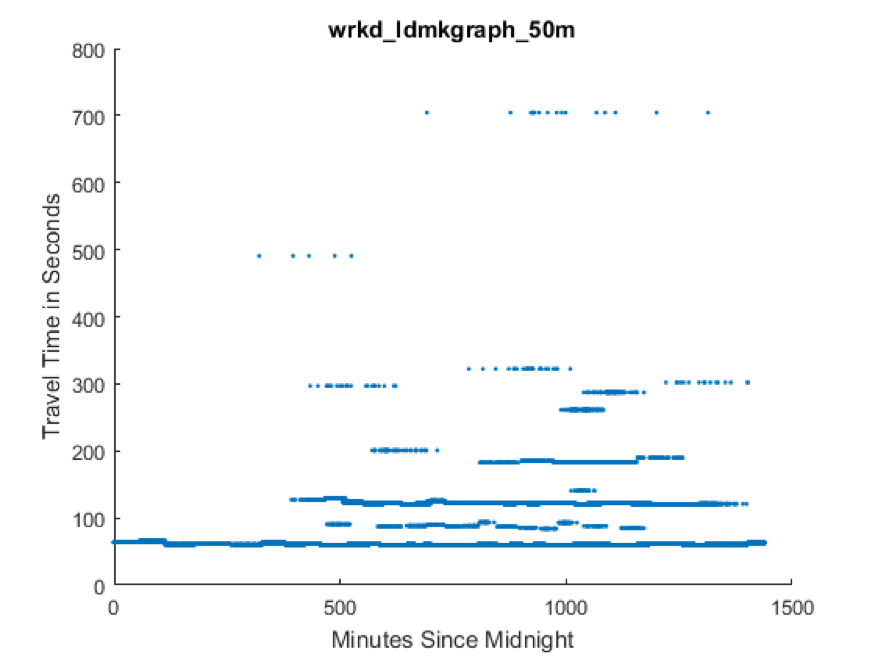
\includegraphics[scale=0.85]{trvltime_neurons}
\centering
\caption{An example of representing data points with centroids}\label{Fig:trvltime_neurons}
\end{figure}

One merit of SOFM clustering is \emph{feature extraction}. In this case, after the training is completed, the SOFM has learned some features about the travel time at different time of the day and expressed its understanding by moving its neurons to the centroids of the clusters. Now, \textbf{the data points can be represented by their respective centroids}. Figure~\ref{Fig:trvltime_neurons} shows the effect of replacing each data point's value with their centroids'. The clusters are clearly shown by the horizontal lines formed by those centroids. 

Representing data points with cluster centroids or features learned provides the benefit of \emph{generalisation}. The data set used in this project, albeit large in size, is nevertheless a small \emph{sample} of the \emph{population} of taxi trajectories over time. In other words, these trajectory records are only the \emph{observed} ones but there are potentially infinite number of trajectories that cannot be all observed. The only information known about them is that \textbf{they must fit into one of the clusters} after undergoing the same procedures described in the previous chapters. The use of centroids instead of real data points also takes into consideration the unobserved trajectories and reflects the real underlying patterns. In fact, generalisation is an advantage that all neural network-based methods share. 

\begin{figure}[h!]
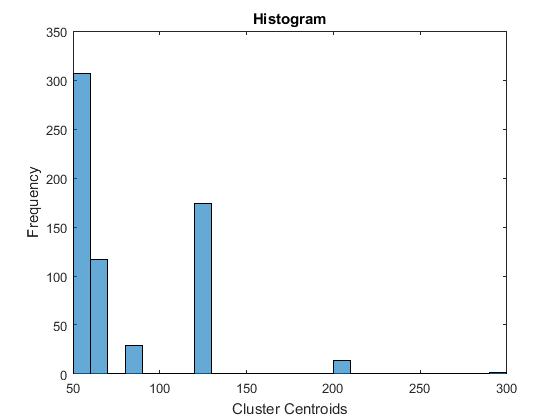
\includegraphics[scale=0.85]{clus_histo}
\centering
\caption{An example of distribution of clusters}\label{Fig:clus_histo}
\end{figure}

Now that the clusters are identified, Figure~\ref{Fig:clus_histo} shows a histogram of clusters within the 10:00~a.m. to 10:30~a.m. interval. It can be observed that within a particular time interval, there are many clusters of travel time and each cluster has different sizes. To describe the travel time pattern within a particular time interval, the histogram is converted into a cumulative probability distribution of clusters which is then fitted with Weibull Distribution described in Theorem~\ref{Theorem: weibull_dist}. 

\begin{theorem}[\emph{Weibull Distribution}]\label{Theorem: weibull_dist}
A Weibull Distribution is described by two strictly positive parameters, the scale parameter $\alpha$ and the shape parameter $\beta$, and has a \textbf{probability distribution function} of \cite{WEDI}
\begin{equation}
f(x | \alpha, \beta) = \frac{\beta}{\alpha}\cdot(\frac{x}{\alpha})^{\beta - 1}\cdot e^{-(x / \alpha)^{\beta}}.
\end{equation}
Correspondingly, its \textbf{cumulative distribution function} is given by \cite{WEIB}
\begin{equation}
F(x | \alpha, \beta) = \int_{0}^{x} f(t | \alpha, \beta) dt = 1 - e^{-(x / \alpha)^{\beta}}.
\end{equation}
\end{theorem}

\begin{figure}[h!]
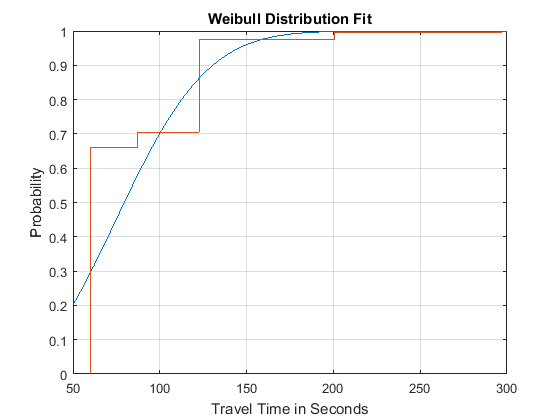
\includegraphics[scale=0.85]{weibull_fit}
\centering
\caption{Weibull Distribution Fit}\label{Fig:weibull_fit}
\end{figure}

Figure~\ref{Fig:weibull_fit} shows an example of fitting a cumulative probability distribution with Weibull Distribution. The red line represents the cumulative probability distribution and the blue line indicates the best Weibull Distribution fit estimated by maximum likelihood. 

In the referencing paper \cite{TDR10}, it uses inverse Gaussian distribution to fit the centroid distribution. However, as some experiments showed, inverse Gaussian distribution does not always work, especially when the centroids actually have a uniform distribution, namely, when only one cluster appears in the time interval. In that case, Weibull distribution will have the shape parameter $\beta = \infty$ but it still can give the correct result. 

The cumulative distribution function of Weibull distribution is good at calculating the probability whereby the travel time $t$ is less than a particular value. For instance, the probability of the travel time for this landmark graph edge being less than or equal to 100 seconds is approximately $P(t\leq100) = 0.7$ according to the Weibull distribution curve in Figure~\ref{Fig:weibull_fit}. But to estimate the travel time of a landmark graph edge is in fact the \emph{reverse}: given a known probability $P$, find the corresponding travel time $t$, which is exactly the inverse Weibull cumulative distribution function does. 

\begin{theorem}[\emph{Inverse Weibull Cumulative Distribution Function}]\label{Theorem: weibull_inverse_dist}
The inverse Weibull cumulative distribution function is defined as
\begin{equation}
F^{-1}(x | \alpha, \beta) = G(p) = \alpha(-ln(1 - p)) ^ {1/\beta}
\end{equation}
where $p$ is the given probability.
\end{theorem}

In practice, the probability $p$ corresponds to some subjective measures of a driver's driving skill. It represents how fast a driver drives as compared to other drivers. If a driver has a $p$ value of 0.2, it means that this driver usually drives faster than 80\% ($1 - 0.2$) drivers. This concept is formally defined in Definition~\ref{Def:opti_index}.

\begin{defn}[\emph{Optimism Index}]\label{Def:opti_index}
A optimism index $p$ indicates how optimistic a driver feels about his or her driving skills \cite{TDR10}. A driver with an optimism index of $p_{0}$ usually drives faster than $(1 - p_{0})\%$ drivers. 
\end{defn}

The optimism index of a driver can be set by the driver in advance, although it may be subject to illusory superiority\footnote{In a 1986 experiment, \emph{80\%} participants rated their driving skills \emph{above-average} \cite{IFD86}.}. It can also be set to the mean value by default or learned from the driver's trajectory history. 

With optimism index defined, it is easy to estimate the travel time using Theorem~\ref{Theorem: weibull_inverse_dist}. However, it is worth mentioning that for a cumulative probability distribution function $F(x)$, the probability of a single value is zero, namely, $F(x_{0}) = 0$; only a range of values can have positive probabilities. Therefore, the travel time calculated from optimism index should really be a \emph{range} of travel time. For instance, if the optimism index is $p = 0.7$, the correct result should be $t \leq 100$ based on Figure~\ref{Fig:weibull_fit}, which means that for a driver with an optimism index of 0.7, his or her travel time is \emph{at most} 100 seconds. No exact value can be determined. However, in the context of this project, only the \emph{worst-case} travel time is considered; therefore, the driver is said to have an expected travel time of 100 seconds. 

\section{Travel Time Evaluation}
After the travel time distributions for each significant edge were determined, an eva\-luation was conducted to ascertain the accuracy of the travel time estimates. In this project, the estimates made by Theorem~\ref{Theorem: weibull_inverse_dist} were compared against real-time estimates made by Baidu Maps at various times of the day. 

Some complications do arise, however, because the two vertices of each significant edge are actually two \emph{landmarks}. Definition~\ref{Def:ldmk} states that a landmark is essentially a road segment with its length ignored. But in estimating the travel time between two landmarks, the length of the landmarks cannot be ignored and has profound effects on how the travel time should be calculated. 

\begin{figure}[h!]
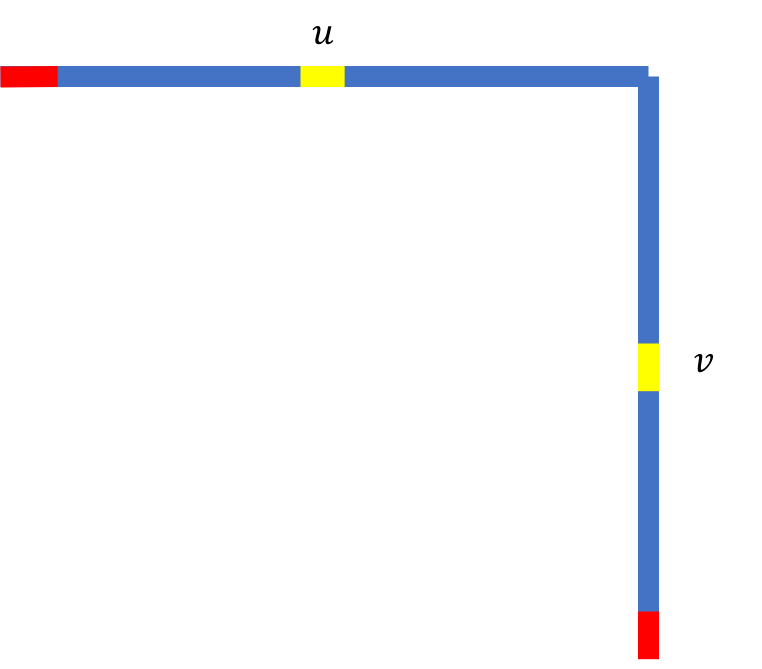
\includegraphics[scale=0.8]{ldmk_travel}
\centering
\caption{An example of different landmark travel time}\label{Fig:ldmk_travel}
\end{figure}

Imagine there are two landmarks $u$ and $v$, respectively, and each has a length of $L$ as shown in Figure~\ref{Fig:ldmk_travel}. Then, there are potentially infinite number of ways of `traveling from $u$ to $v$', because the starting point could be any points on $u$ and the ending point could be any points on $v$. If a driver starts at the red point on $u$ and stops at the red point on $v$, the total distance is $2L$ and the total time is $T$. But had the driver stopped at the yellow mid-point on $v$, the total distance would be $1.5L$ and the total time would be $3T/4$, assuming the speed is constant. 

Therefore, it is difficult to give a \emph{definite} estimate of the travel time between two landmarks. In this project, the \textbf{median travel time} is instead used to represent the travel time between two landmarks. It describes the \emph{typical} travel time a driver should expect. An example of a median case is that the diver starts at the yellow mid-point on $u$ and ends at the yellow mid-point on $v$. But there are in fact infinite number of median cases. 

The most significant 150 edges were selected to be evaluated, from \emph{each} of the four landmark graphs listed in Table~\ref{Ta:ldmkgraphs}. For each edge $(u, v)$, 20\% of the trajectories with $u$ as starting point and $v$ as ending point were randomly sampled. These trajectories represent some random trips between $u$ and $v$ with varying distances. Baidu Maps API was then used to estimate the travel time for each trajectory in real time, after which the median of all the estimates was selected as Baidu's estimate for the travel time between $u$ and $v$. Finally, Theorem~\ref{Theorem: weibull_inverse_dist} was used to calculate its own the travel time estimate which was then compared against Baidu's. Table~\ref{Ta:eval_res} summarises the evaluation results for all 150 significant edges. 

\begin{table}[h!]
\centering
\resizebox{\columnwidth}{!}{
\begin{tabular}{ | c | c | c | c |}
\hline
\textbf{Landmark Graph} & \textbf{RMSE} & \textbf{Mean Error Ratio} & \textbf{Mean No. of Samples Per Edge} \\ \hline
wrkd\_ldmkgraph\_50m & 78.58 & -0.009 & 1824.60 \\ \hline
wrkd\_ldmkgraph\_30m & & & 1507.56 \\ \hline
holi\_ldmkgraph\_50m & 87.39 & -0.16 & 832.96 \\ \hline
holi\_ldmkgraph\_30m & 76.41 & -0.14 & 681.89 \\ \hline
\end{tabular}}
\caption{Summary of Evaluation Results}\label{Ta:eval_res}
\end{table}

Assuming a Baidu's estimate is $b_{i}$ and the corresponding project's estimate is $\hat{b}_{i}$, then the Root Mean Square Error (RMSE) is given by:
\begin{equation}
RMSE = \sqrt{\frac{\sum_{i = 1}^{N}(\hat{b}_{i} - b_{i})^{2}}{N}}
\end{equation}
where $N$ is the total number of estimates; and the Mean Error Ratio (MER) is given by:
\begin{equation}
MER = \frac{1}{N}\sum_{i = 1}^{N}\frac{\hat{b}_{i} - b_{i}}{b_{i}}
\end{equation}

The RMSE gives an overall measure of accuracy. For instance, the RMSE for landmark graph \emph{wrkd\_ldmkgraph\_50m} turned out to be 78.58, which means that on average, the difference between Baidu's estimates and Theorem~\ref{Theorem: weibull_inverse_dist}'s estimate was 78.58 seconds. But whether this difference is significant or not depends on the scale of Baidu's estimates. For a Baidu's estimate of 30 seconds, 78.58 seconds may be considered significant, but for an estimate of 200 seconds, it may be acceptable. 

Therefore, MER is designed to take into account the scale of Baidu's estimates. It computes the ratio between the error and Baidu's estimate. A positive MER indicates that on average Theorem~\ref{Theorem: weibull_inverse_dist} tends to have larger estimates than Baidu's; on the other hand, a negative MER indicates that on average, Theorem~\ref{Theorem: weibull_inverse_dist} tends to have smaller estimates than Baidu's. 

Another technique to gauge Theorem~\ref{Theorem: weibull_inverse_dist}'s performance is linear regression. An ordered pair of estimates $(b_{i}, \hat{b}_{i})$ can be treated as a point in a 2-D Cartesian system. In the \emph{ideal} case, $\hat{b}_{i}$ should be equal to $b_{i}$, therefore, all points should form a straight line with a slope of 1 and an intercept of 0 when plotted. In the general cases, linear 
